\subsection{Flash Loans}
Flash loans are zero-risk loans which enables anyone to borrow large amounts of money, which they can do what they please with, as long as they pay the loan back within the same transaction. This will sound crazy to the uninitiated but lets explain. Usually there is a risk in lending money, that is the risk of the borrower not paying it back, however this can be gaurenteed by the blockchain. When a transaction is being computed it can be rolled back if something invalidates the transaction, so if we say that not repaying the loan is in violation of the contract, then the block will role back to before the transaction.

When taking a flash loan you borrow from a liquidity pool, and when borrowing from this pool you pay back a fee thereby incentivizing individuals and investors to deposit in the pool.

\subsection{Terminology alert}
\subsubsection{Dencentralized exchange (DEX)}
A dencentralized exchange is (like normal exchanges) a service where actors can exchange their assets in a dencentralized fashion.

\paragraph{Limit order book (LOB)}
A limit order book is a record of so called \textit{limit orders}. A limit order is a trader requesting to buy or sell up to a certian price, so if we want to sell an (or multiple) assets a limit order could be that we want to sell asset X at 15\$ or higher, or if we were buying we would say that we want to buy asset X at 15\$ or below. A LOB is simply a record of such limit orders. An example of this can be seen in figure
\begin{figure}[h]
  \centering
  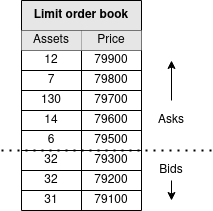
\includegraphics[width=0.3\textwidth]{assests/Flash-loans-LOB}
  \caption{A visual example of a limit order book.}
  \label{fig:LOB}
\end{figure}

\paragraph{Automated market maker (AMM)}
We have specifically looked at Uniswap when understanding AMM's, so while this definition will fit most AMM's since we look at the concept, the math/implementation of the concept might differ from AMM to AMM.

AMM's works by exchanging assets between pools in a contract, for example one contract could exchange DAI for BTC then this contract wil contain a pool of DAI and a pool of BTC. This method is how Uniswap version 2 works, here we have a great number of contracts since we have a contract for each exchange pair, so one for DAI/BTC, one for DAI/LTC etc. Version 1 of Uniswap worked by having ETH as the "background" currency meaning that for each asset (X) there was a contract containing ETH and X, you could then exchange ETH to X and X to ETH but if you wanted to swap Y for X you would need to swap Y for ETH, and ETH for X. This is not good since you trade twice, and encur the fees associated with that twice, as well as experiencing the \textit{slippage} in both trades, and this is one of the things that the second version of the Uniswap protocol fixes.

\paragraph{Slippage} We have an overview of how AMM's work, but unlike LOB's it is not clear how we determine the exchange rate between asset X and asset Y.


, so if you fx. have a pair of pools A/B then you will have the relationship A*p=c where c is some constant set at the start. So if pool A is 100 a’s and c is 20.000 then you have that 1 a costs 100 b’s, if 1 a is now traded from the pool, A becomes 99 and the new price is approx 202.